\documentclass[letterpaper,10pt,conference]{ieeeconf}
\IEEEoverridecommandlockouts
\overrideIEEEmargins

\usepackage{amsmath,amssymb,booktabs,cite}
\usepackage[T1]{fontenc}
\usepackage{mathptmx,graphicx,microtype,url}
\usepackage[dvipsnames]{xcolor}

\newcommand{\model}{YOLO11-DLA-n}
\title{\LARGE\bf Fallback-Free Is Not Free: Accuracy, Latency, and Energy\\
Costs of Full DLA Placement for YOLO11}

\author{Anonymous Authors}
% \author{Alexandru Cretu$^{1}$, Jaleh Farmani$^{1,2}$, Roberto Masocco$^{1}$, Alessandro Tenaglia$^{1}$, Simone Mattogno$^{1}$ and Daniele Carnevale$^{1}$%
% \thanks{
%     Corresponding author: {\tt\small roberto.masocco@uniroma2.it}.\hfill\break
%     $^{1}$Dipartimento di Ingegneria Civile e Ingegneria Informatica,
%         Università degli Studi di Roma Tor Vergata, Via del Politecnico 1, 00133 Rome, Italy}%
% }

\begin{document}
\maketitle

\thispagestyle{empty}
\pagestyle{empty}

\begin{abstract}
Embedded robots share compute resources across perception, localization,
mapping, planning, and control. Requesting execution on NVIDIA's Deep Learning
Accelerator (DLA) can leave learned layers on the GPU. This work asks what it costs to run a modern detector entirely on a
constrained accelerator. On Jetson AGX Orin, a fully DLA-admissible YOLO11
executes inference faster than the same network on GPU in INT8 (4.522 versus
6.400\,ms), yet the native-layout boundaries around it have stage medians of
7.463 and 10.729\,ms, and the application pipeline ends up slower and slightly more
energy-hungry.
Full admissibility requires C2DLA to replace spatial attention with channel softmax and depthwise convolution, together with a static raw prediction boundary for host-side decoding. With TensorRT 10.3, fallback-disabled
compilation and engine inspection confirm one DLA loadable without GPU-assigned
learned layers for the nano model in FP16 and mixed INT8 configurations.
On 4,500 COCO validation images excluded from calibration,
strict DLA achieves 37.876 AP in FP16 and 35.408 AP in INT8; the corresponding
adapted GPU engines achieve 37.879 and 35.951 AP. At batch one and
$640\times640$, INT8 reduces strict DLA median engine-plus-transfer latency
from 27.515 to 4.167\,ms and application-pipeline latency from 56.820 to
30.675\,ms. Module energy at 10\,Hz decreases from 0.874 to 0.806\,J/frame.
The adapted INT8 GPU engine remains faster and lower-energy, at 18.212\,ms
application-pipeline latency and 0.760\,J/frame. The case study shows that
DLA compatibility must be evaluated together with accuracy, host-side processing,
and module energy. Faster accelerator execution alone is not enough to select
a deployment.
\end{abstract}

% \begin{keywords}
% Embedded Systems for Robotic and Automation;
% Hardware-Software Integration in Robotics;
% Deep Learning for Visual Perception.
% \end{keywords}

\section{Introduction}
\label{sec:introduction}
Embedded robots run perception, localization, mapping, planning, and control
on shared compute resources. Platforms with CPUs, GPUs, and dedicated neural
accelerators offer several places to run a detector. Using an accelerator
requires checking which parts of the detector actually run on it.

Nominal DLA deployment differs from verified fallback-free placement of the
learned graph. TensorRT can request DLA execution while allowing unsupported
regions to run on GPU \cite{nvidia_dla_working}. Operator support, tensor shapes,
normalization axes, precision, and I/O layouts constrain placement. A successful
export or a DLA build option alone cannot show where the learned layers execute.

The question is what full DLA placement of a modern detector costs, and where
that cost falls. YOLO11
\cite{jocher2024yolo11} serves as the case study. Its architecture combines a convolutional backbone and neck with spatial self-attention and a decoded prediction interface.
These expose two parts of the deployment problem: incompatible learned
operations and the boundary between the accelerator graph and detection processing.

\begin{figure}[t]
    \centering
    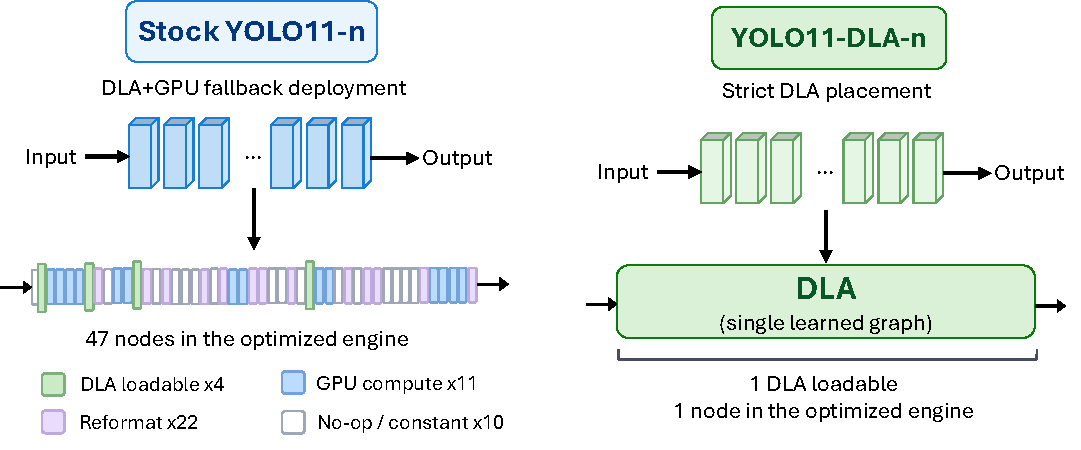
\includegraphics[width=\columnwidth]{figures/teaser.pdf}
    \caption{FP16 deployment. Stock YOLO11-n uses DLA+GPU fallback;
    YOLO11-DLA-n places the complete learned graph in one DLA loadable.
    Host-side decoding and non-maximum suppression remain outside the accelerator.}
    \label{fig:teaser}
\end{figure}

The workflow starts by inspecting the detector and its exported graph, then
attempting strict DLA compilation. The strict compilation failure identifies the blocking learned computation, while the desired accelerator boundary guides the output-interface change. In YOLO11, the attention block forms a spatial affinity matrix through a query--key MatMul that strict DLA compilation rejects. The stock detection head also performs DFL expectation, grid decoding, sigmoid, flattening, and cross-scale concatenation inside the exported graph. Section~\ref{sec:method} replaces the incompatible attention computation with C2DLA and moves the prediction boundary earlier through DetectDLA, which exports three static raw prediction maps. The adapted graph is then compiled with GPU fallback disabled,
and the optimized engine is inspected (Fig.~\ref{fig:teaser}). Host-side decoding,
confidence filtering, and non-maximum suppression (NMS) complete the detector.
The resulting nano model is denoted \model.
The anonymous model implementation is available at \url{https://anonymous.4open.science/r/ultralytics-dla}; the export, deployment, benchmarking, evaluation code, and trained weights are available at \url{https://anonymous.4open.science/r/yolo11_dla}.

\begin{figure*}[t]
\centering
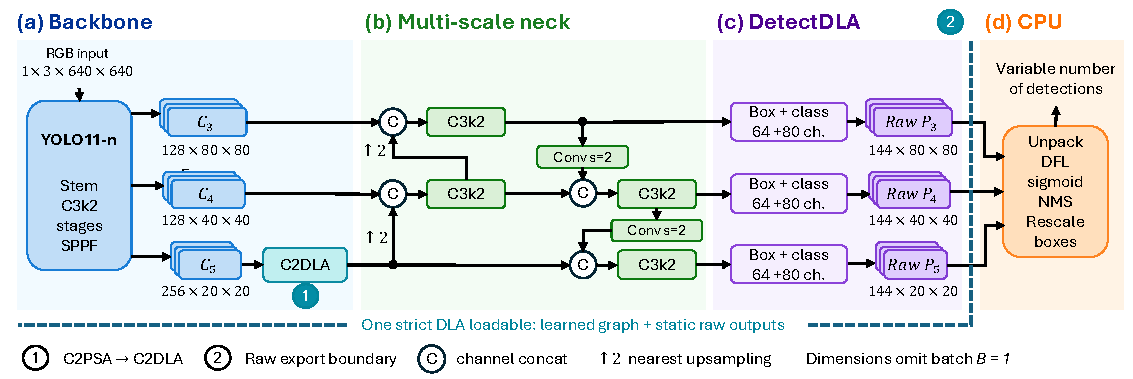
\includegraphics[width=\textwidth]{figures/architecture_overview.pdf}
\caption{\textbf{YOLO11-DLA-n architecture.} Backbone scales feed the neck and box/class
 towers at strides 8, 16, and 32. Markers 1 and 2 identify C2DLA and the raw-output
 boundary. The learned graph forms one DLA loadable; unpacking and post-processing
 remain on CPU. Preprocessing and input packing precede the graph.}
\label{fig:boundary}
\end{figure*}

This work makes three contributions:
\begin{itemize}
\item A modern detector made fully DLA-admissible still runs as one DLA
loadable with no GPU-assigned learned layer, in FP16 and in INT8: fallback-disabled
compilation and optimized-engine inspection verify the placement, which C2DLA
and DetectDLA obtain while retaining the surrounding backbone, neck, detection
towers, and training formulation.
\item The accuracy cost of full placement is negligible in FP16 and non-zero in
INT8. Strict DLA scores $-0.003$ AP in FP16 and $-0.543$ AP in INT8 against the
same network on GPU: the precision regime, not the placement, dominates the
accuracy loss.
\item Latency and energy reverse at the application boundary, and the cause is
measured. In INT8 the inference stage is faster on strict DLA than on the adapted
GPU engine (4.522 versus 6.400\,ms), while the native-layout input and output
boundaries have stage medians of 7.463 and 10.729\,ms, and the adapted GPU configuration remains
faster and lower-energy over the whole pipeline.
\end{itemize}

Moving the learned detector away from GPU compute motivates this study, but concurrent workloads are not evaluated. The evidence here covers the YOLO11 case study on the tested
Orin/TensorRT configuration.

\section{Related Work}
\label{sec:related}
\paragraph*{Efficient object detection}

YOLO evolved from single-network detection \cite{redmon2016yolo} through
multi-scale prediction and feature/training refinements
\cite{redmon2018yolov3,bochkovskiy2020yolov4}, anchor-free heads and assignment
\cite{ge2021yolox}, deployment-oriented structures \cite{li2022yolov6},
training and aggregation improvements \cite{wang2023yolov7,wang2024yolov9},
and NMS-free prediction \cite{wang2024yolov10}. These developments motivate
YOLO11 as a representative detector; GPU benchmarks alone do not show
complete DLA placement. YOLO11's detection towers and distributional
regression are retained \cite{jocher2024yolo11,li2020gfl}. Its surrounding
structure draws on feature partitioning and pyramid aggregation
\cite{wang2020cspnet,lin2017fpn,liu2018panet}. Unlike RepVGG-style deployment
re-parameterization \cite{ding2021repvgg,li2022yolov6}, the proposed adaptation changes
the incompatible attention computation while preserving this surrounding
structure. The objective is accelerator-compatible deployment rather than
optimization of the AP/FLOPs trade-off.

\paragraph*{Hardware-aware and edge network design}

YOLO-ReT and YOLOBench address edge-GPU detection and controlled evaluation
across embedded hardware \cite{ganesh2022yoloret,lazarevich2023yolobench};
ActNAS examines hardware-sensitive activation choices \cite{sah2025actnas};
NAS and co-design methods incorporate target latency or runtime into model
selection \cite{tan2019mnasnet,cai2019proxyless,cai2020ofa,lin2020mcunet}.
Here strict compilation is a feasibility constraint for a manually specified
adaptation. C2DLA uses projection and normalization related to external attention
\cite{guo2023external}, but only mixes channels at each position and adds local
depthwise context.

\paragraph*{Heterogeneous accelerator deployment for embedded perception}
Archet et al.\ \cite{archet2023energy} study CNN design and inference options
on Jetson AGX Orin, showing that its CPU, GPU, and DLA offer different latency
and energy trade-offs. Hern\'andez et al.\ \cite{hernandez2024optimizing}
evaluate quantization on AGX Orin and report that DLA layer incompatibilities
degrade inference performance and efficiency in their tested models.
These studies make network compatibility part of the practical
accelerator-selection problem.

Tayal and Simmhan \cite{tayal2024multiinstance} examine multi-instance inference
across Orin's CUDA cores, Tensor Cores, and DLAs, investigating resource
congestion under concurrent workloads. Chakraborty et al.\
\cite{chakraborty2025profiling} profile concurrent vision inference on Jetson,
linking throughput degradation to resource contention and CPU--GPU scheduling;
aggregate GPU utilization alone does not describe component-level efficiency.
These findings motivate explicit workload placement in robotic systems.

Compiler lowering \cite{chen2018tvm} and TensorRT's optional GPU fallback
\cite{nvidia_dla_working} make compatibility an architectural and deployment
property, not merely an exporter setting. This case study combines these steps in one deployment workflow and evaluates the resulting accuracy, latency, and energy.

\section{YOLO11-DLA-n: Adaptation and Design}
\label{sec:method}
\begin{figure*}[t]
\centering
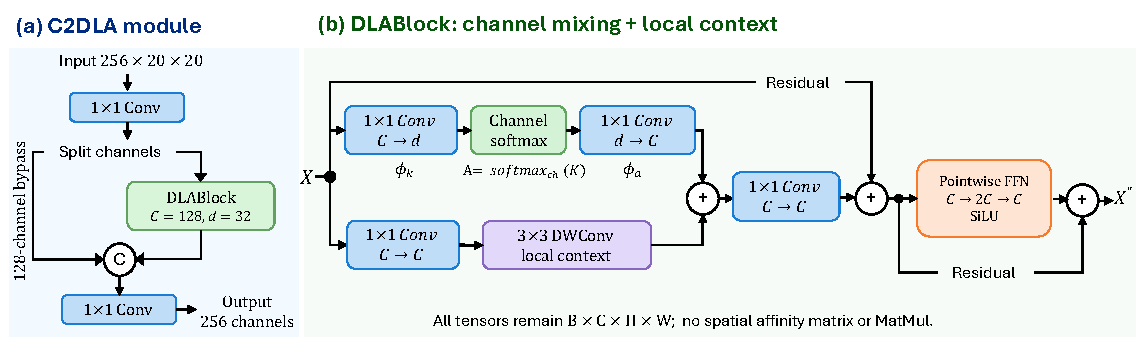
\includegraphics[width=\textwidth]{figures/c2dla_detail.pdf}
\caption{\textbf{C2DLA module and operators.} (a) Nano-model split--process--merge block
 at $20\times20$. (b) Channel softmax and local depthwise convolution replace spatial
 attention, retaining both residual additions and the pointwise FFN.
 C denotes concatenation; $+$ denotes elementwise addition.}
\label{fig:c2dla}
\end{figure*}
\subsection{Design Objective and Verification Criterion}
The workflow treats learned-graph placement as a deployment constraint.
Let $G$ denote the learned graph obtained by adapting the reference YOLO11-n graph.
The objective is to obtain a useful detector whose complete learned computation can run on the tested DLA configuration:
\begin{equation}
 \operatorname{Build}_{\mathrm{DLA}}(G;\theta,\mathrm{fallback}=0)
 = E, \qquad N_{\mathrm{GPU}}(E)=0,
 \label{eq:accept}
\end{equation}
where $\theta$ fixes the target, compiler version, precision, shapes, and
I/O formats, $E$ is the serialized engine, and $N_{\mathrm{GPU}}$ counts
GPU-assigned learned layers after optimization. For this YOLO11 case study, the target is also a single DLA loadable. These are deployment criteria, not training
loss terms. Accuracy and application performance are then evaluated separately.

\subsection{Compatibility Analysis and Adaptation}
Inspection of stock YOLO11-n identifies spatial attention and a flattened, decoded output interface. C2PSA is YOLO11's attention block. It uses a split--process--merge structure in which one branch applies spatial self-attention over the $20\times20$ feature map. This attention requires a query--key MatMul, which strict FP16 compilation rejects. Replacing that learned computation removes the reported blocker. Separately, exporting static raw predictions places the accelerator boundary before decoding and cross-scale output processing. The adaptation therefore uses two substitutions:
\begin{equation}
 \mathrm{C2PSA}\longrightarrow\mathrm{C2DLA},\qquad
 \mathrm{Detect}\longrightarrow\mathrm{DetectDLA}.
 \label{eq:substitutions}
\end{equation}
The surrounding convolutional stem, C3k2 stages, SPPF module, feature-pyramid
connections, detection towers, and ordinary training path are retained
(Fig.~\ref{fig:boundary}). The adapted GPU engine serves as a same-model
placement control. Comparisons with stock YOLO11-n also include architecture,
training, and prediction-interface differences.

\subsection{C2DLA: Replacing Incompatible Spatial Attention}
\label{sec:c2dla}
The replacement must mix information within the processed branch without forming a spatial affinity matrix. C2DLA does this with channel-wise softmax and local depthwise convolution while retaining C2PSA's surrounding split--process--merge structure (Fig.~\ref{fig:c2dla}). An initial $1\times1$
projection produces two channel groups; one bypasses the inner block and the
other is processed before concatenation and a final projection. If $X$ is the
processed group with $C$ channels, define
\begin{align}
 K &= \phi_k(X), \qquad V=\phi_v(X), \label{eq:kv}\\
 A_{bkhw} &= \frac{\exp K_{bkhw}}{\sum_{j=1}^{d}\exp K_{bjhw}},
 \label{eq:chansoftmax}\\
 Z &= \phi_o\bigl(\phi_a(A)+\psi_{3\times3}(V)\bigr),
 \label{eq:mix}\\
 X' &= X+Z, \label{eq:res1}\\
 X'' &= X'+\operatorname{FFN}(X'). \label{eq:res2}
\end{align}
Here $d=\max(\lfloor C/4\rfloor,8)$; $\phi_k:C\to d$,
$\phi_v:C\to C$, $\phi_a:d\to C$, and $\phi_o:C\to C$ are
$1\times1$ projections. The operator $\psi$ is a $3\times3$ depthwise
convolution. The FFN expands channels from $C$ to $2C$, applies SiLU, and
projects back to $C$. Batch normalization accompanies the relevant convolution
modules and is folded into them for inference; $\phi_a$ is a bias-free
convolution without batch normalization.

The nano configuration is shown in Fig.~\ref{fig:c2dla}: one inner block at the
$20\times20$ scale with $C=128$ and $d=32$. No operation introduces matrix
multiplication, head transposes, or normalization over image positions.

The block uses input-dependent channel mixing and local depthwise context.
It does not model long-range spatial affinities. It changes the hypothesis class
and is not algebraically equivalent to C2PSA; greater representational power
is not claimed. Its accuracy is evaluated in Section~\ref{sec:accuracy}.

\subsection{DetectDLA: A Static Prediction Boundary}
\label{sec:boundary}
Stock Detect performs the expectation over the discrete regression distribution used by distribution focal loss (DFL), grid decoding, sigmoid, flattening, and cross-scale concatenation inside the exported graph before producing its fixed decoded output. DetectDLA stops earlier and instead exposes the three raw multi-scale prediction maps, leaving these operations and variable-cardinality filtering and NMS to the host.

For each pyramid level $\ell\in\{3,4,5\}$, the retained regression and
classification towers produce $R_\ell$ and $S_\ell$. DetectDLA exports
\begin{equation}
 P_\ell=\operatorname{Concat}_{C}(R_\ell,S_\ell)
 \in\mathbb{R}^{B\times(4r+n_c)\times H_\ell\times W_\ell},
 \label{eq:packed}
\end{equation}
with $r=16$ regression bins and $n_c=80$ COCO classes. For batch one and
$640\times640$ images, the outputs are $1\times144\times80\times80$,
$1\times144\times40\times40$, and $1\times144\times20\times20$ at strides
8, 16, and 32. They are named \texttt{pred\_p3}, \texttt{pred\_p4}, and
\texttt{pred\_p5}. Classification values are logits; box channels are
unnormalized distributions, not decoded coordinates.

During training and ordinary PyTorch inference, DetectDLA invokes the
inherited Detect path, retaining its losses and assignment behavior. The change
concerns deployment partitioning, not a direct-regression or one-to-one
prediction formulation.

At FP16, the adapted raw output is $1.714\times$ larger than the stock decoded
output, increasing transfer and host-decoding work.

\subsection{Training and Initialization}
The adapted model is initialized from pretrained YOLO11-n weights. Parameters
with matching names and shapes are reused, while unmatched replacement
parameters retain their initialization; all trainable layers are then fine-tuned.
Training uses COCO train2017 for 500 epochs with batch size 32, $640\times640$
inputs, automatic mixed precision (AMP), and standard HSV, geometric,
horizontal-flip, and mosaic augmentation. Stock and adapted models were not
trained with equal budgets, so their comparison evaluates the resulting
deployed detectors rather than an isolated architectural substitution.

\section{Export and Runtime}
\label{sec:deployment}
\subsection{Exported Graph and Strict Compilation}
The adapted model is exported with a static $1\times3\times640\times640$ input.

Strict compilation targets DLA core 0 in FP16 and calibrated INT8, with GPU
fallback disabled and explicit native I/O formats. Optimized-engine inspection
confirms that each strict engine contains a single DLA node corresponding to
one loadable. DLA operator support depends on the target and TensorRT version
\cite{nvidia_dla_working}.

\subsection{Native Layouts and the Host Boundary}
\label{sec:packing}
Strict FP16 uses DLA\_HWC4 input and CHW16 outputs; strict INT8 uses
DLA\_HWC4 input and CHW32 outputs \cite{nvidia_dla_working}.
GPU and stock DLA+GPU fallback engines retain linear FP16 external bindings
in both precision modes. For native INT8 bindings, the host uses per-tensor
scales to quantize input pixels and dequantize raw outputs.

The application runner performs packing, unpacking, and INT8 conversion on the
CPU. Timed input stages include packing and host-to-device (H2D) transfer;
output stages include device-to-host (D2H) transfer, unpacking, and any
dequantization.

\subsection{Confidence-First Host Decoding}
\label{sec:decode}
The host splits each $P_\ell$ into 64 regression channels and 80 class channels.
For confidence threshold $\tau\in(0,1)$, an anchor survives if
\begin{equation}
 \sigma\!\left(\max_c S_{\ell,c}(h,w)\right) > \tau.
 \label{eq:threshold}
\end{equation}
For each survivor and box side $q\in\{l,t,r,b\}$, the DFL expectation is
\begin{equation}
 \hat d_q=\sum_{j=0}^{r-1}j\,
 \frac{\exp R_{qj}}{\sum_{k=0}^{r-1}\exp R_{qk}}.
 \label{eq:dfl}
\end{equation}
The decoder places cell centers at $(w+0.5,h+0.5)$, forms the four box
coordinates from these distances, scales by the level stride, applies class
sigmoid, and performs class-aware NMS. The final coordinates are mapped back
through the image's letterbox transform.

Regression decoding is applied only to candidates that pass the confidence
test; this reduces host decoding work but does not reduce raw-output transfer volume.

\section{Experimental Evaluation}
\label{sec:eval}
The evaluation checks whether the adaptation achieves strict DLA placement, what accuracy is retained, and how precision affects engine-plus-transfer latency, application-pipeline latency, and host-side cost. Module energy is measured separately at a matched 10\,Hz delivered rate. Each precision mode
includes stock YOLO11-n on GPU and with DLA+GPU fallback (stock fallback), and \model\ on GPU
and strict DLA. In the tables, DLA denotes strict placement for the adapted model.
Because \model\ on GPU and \model\ on strict DLA share the same weights, host
decoder, and NMS implementation, their difference isolates placement;
comparisons involving stock YOLO11-n also include architecture, training, and
prediction-interface differences.

\subsection{Platform and Precision Protocol}
\label{sec:setup}
Tests use an NVIDIA Jetson AGX Orin Developer Kit with L4T 36.4.4, CUDA 12.6,
and TensorRT 10.3 in NVIDIA's 50\,W mode with \texttt{jetson\_clocks} disabled.
All configurations use batch one and $640\times640$ inputs. FP16 enables
half precision; INT8 enables mixed INT8/FP16. These are build modes rather
than uniform operation precisions; GPU regions may retain FP16/FP32 intermediates.

Post-training calibration uses 500 COCO val2017 images sampled without
replacement with seed 2027, leaving 4,500 disjoint images for accuracy
\cite{lin2014coco}. Stock and adapted models are calibrated separately with
TensorRT's EntropyCalibrator2 using the same calibration image IDs.
INT8 entails no additional training.

\begin{table*}[!t]
\caption{Deployment latency at the engine and application boundaries, batch one, $640\times640$. All values are milliseconds. Engine measurements include transfers (30\,s); application measurements include preprocessing, native I/O, inference, decode, and NMS over a 60\,s application run.}
\label{tab:latency}\centering\footnotesize
\setlength{\tabcolsep}{4pt}
\begin{tabular*}{\textwidth}{@{\extracolsep{\fill}}lllrrrr@{}}
\toprule
& & & \multicolumn{2}{c}{Engine + transfer} & \multicolumn{2}{c}{Application} \\
\cmidrule(lr){4-5}\cmidrule(l){6-7}
Model & Device & Mode & Median & P95 & Median & P95 \\
\midrule
YOLO11-n & GPU & FP16 & 3.740 & 3.753 & 20.030 & 24.658 \\
YOLO11-n & DLA+GPU & FP16 & 34.678 & 34.942 & 51.241 & 59.542 \\
YOLO11-DLA-n & GPU & FP16 & 3.500 & 3.512 & 20.307 & 24.584 \\
YOLO11-DLA-n & DLA & FP16 & 27.515 & 27.718 & 56.820 & 65.042 \\
\midrule
YOLO11-n & GPU & INT8 & 3.021 & 3.030 & 17.556 & 22.104 \\
YOLO11-n & DLA+GPU & INT8 & 13.068 & 13.094 & 29.020 & 37.510 \\
YOLO11-DLA-n & GPU & INT8 & 2.828 & 2.836 & 18.212 & 22.467 \\
YOLO11-DLA-n & DLA & INT8 & 4.167 & 4.173 & 30.675 & 34.812 \\
\bottomrule
\end{tabular*}
\end{table*}

\subsection{Fallback-Free Placement}
\label{sec:placement}
Stock YOLO11-n fails strict compilation in both FP16 and INT8. The
adapted FP16 build assigns 299 layers to DLA and none to GPU. Both adapted
strict engines have one optimized DLA node corresponding to one loadable,
with no GPU or reformat nodes. The INT8 build assigns 298 layers to INT8 and
one softmax to FP16, all on DLA. Fallback-disabled compilation and inspection
therefore satisfy Eq.~\eqref{eq:accept} in both modes. The strict INT8 engine
uses mixed precision entirely within its DLA loadable.

\begin{figure}[!t]
\centering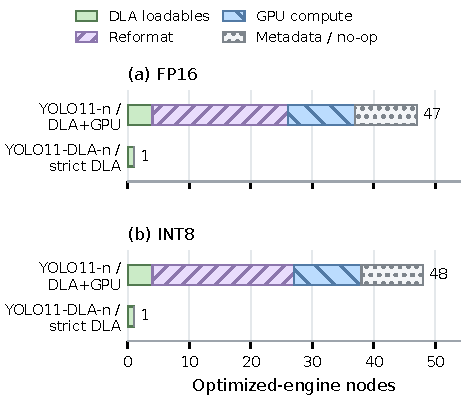
\includegraphics[width=\columnwidth]{figures/engine_composition.pdf}
\caption{Optimized-engine composition in FP16 and INT8. Counts are taken from
TensorRT engine-inspector outputs and represent DLA loadables, reformat nodes,
GPU compute nodes, and metadata/no-op nodes. In both precisions, YOLO11-n with
DLA+GPU execution remains partitioned across four DLA loadables with interleaved
GPU and reformat nodes, whereas strict YOLO11-DLA-n forms one DLA loadable with
no GPU or reformat nodes. These counts describe optimized-engine nodes, not
source-layer assignments or profiler records.}
\label{fig:composition}
\end{figure}

Figure~\ref{fig:composition} shows that the optimized-engine structure is nearly
unchanged by precision. YOLO11-n with DLA+GPU execution contains four DLA
loadables, eleven GPU compute nodes, and 22/23 reformat nodes in FP16/INT8,
whereas strict \model\ remains one DLA loadable with no GPU or reformat nodes
in both modes.
Comparing these heterogeneous deployments with strict DLA includes changed
attention and output boundaries and does not isolate partitioning cost.

\subsection{Engine-Plus-Transfer Latency}
\label{sec:engine}
The \texttt{trtexec} microbenchmark uses a 2\,s warm-up, a 30\,s timing window,
one inference stream, spin waiting, generated input data, and transfers enabled:
\begin{equation}
 L_{\mathrm{engine+IO}}=T_{\mathrm{H2D}}+T_{\mathrm{device}}+T_{\mathrm{D2H}}.
 \label{eq:latency}
\end{equation}
This boundary excludes preprocessing, host-side decoding, and NMS.
The reported percentiles describe frame variation within
each test, not confidence intervals across independent trials.

Table~\ref{tab:latency} shows that INT8 reduces strict DLA
median engine-plus-transfer latency from 27.515 to 4.167\,ms, a $6.60\times$ speedup. Strict DLA has lower
engine-plus-transfer latency than stock fallback in both modes: 20.7\% lower
median in FP16 and a $3.14\times$ reduction in INT8. The same adapted model on
GPU remains faster at this boundary: 3.500\,ms in FP16 and 2.828\,ms in INT8. Accuracy and application-pipeline costs are examined next.

\begin{figure*}[!t]
\centering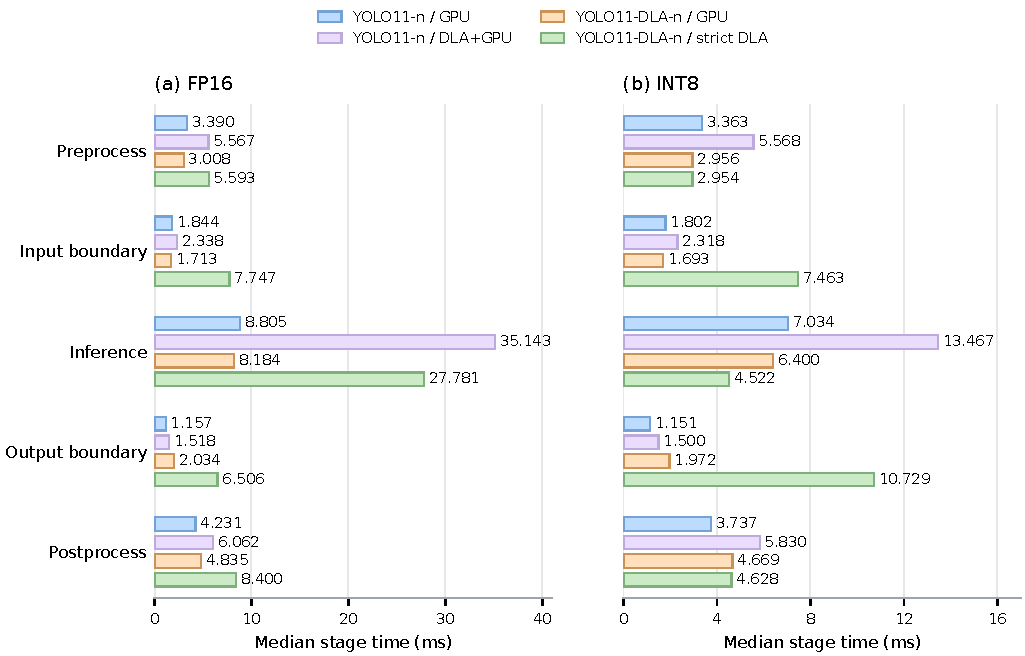
\includegraphics[width=\textwidth]{figures/application_stages.pdf}
\caption{Application-stage medians for all eight configurations under the same application workload. Panels use different horizontal scales. Input boundary
includes packing, quantization where needed, and H2D transfer; output boundary
includes D2H transfer, unpacking, and dequantization where needed. Inference
includes runtime launch and synchronization. Postprocess includes decoding and
NMS. Stage medians do not necessarily sum to the median total latency.}
\label{fig:stages}
\end{figure*}

\subsection{Deployed-Engine Accuracy}
\label{sec:accuracy}
The main comparison evaluates all eight configurations on the same 4,500
held-out images. Preprocessing centers a square $640\times640$ letterbox with padding
114 and RGB normalization by 255. CPU post-processing uses confidence 0.001,
class-aware NMS at intersection over union (IoU) 0.7, multi-label candidates,
and at most 300 boxes per image; COCOeval uses standard detection limits.
These settings differ from the timing thresholds.

\begin{table}[!b]
\caption{Accuracy on 4,500 held-out COCO val2017 images, disjoint from INT8 calibration. AP values are percentage points; INT8 allows mixed precision; stock and adapted training budgets differ.}
\label{tab:accuracy}\centering\footnotesize
\setlength{\tabcolsep}{3pt}
\begin{tabular*}{\columnwidth}{@{\extracolsep{\fill}}lllrrr@{}}
\toprule
Model & Device & Mode & AP & AP$_{50}$ & AP$_{75}$ \\
\midrule
YOLO11-n & GPU & FP16 & 39.378 & 55.190 & 42.845 \\
YOLO11-n & DLA+GPU & FP16 & 39.308 & 55.160 & 42.823 \\
YOLO11-DLA-n & GPU & FP16 & 37.879 & 53.633 & 41.008 \\
YOLO11-DLA-n & DLA & FP16 & 37.876 & 53.614 & 41.016 \\
\midrule
YOLO11-n & GPU & INT8 & 33.175 & 47.324 & 36.069 \\
YOLO11-n & DLA+GPU & INT8 & 19.827 & 35.241 & 20.867 \\
YOLO11-DLA-n & GPU & INT8 & 35.951 & 51.063 & 39.323 \\
YOLO11-DLA-n & DLA & INT8 & 35.408 & 50.790 & 38.614 \\
\bottomrule
\end{tabular*}
\end{table}
Table~\ref{tab:accuracy} compares precision and placement using the same images.
Strict INT8 loses 2.468 AP points relative to strict FP16; adapted GPU loses
1.928 points. Within a precision mode, strict DLA minus adapted GPU AP is
$-0.003$ points in FP16 and $-0.543$ in INT8. Thus, the negligible FP16
placement difference does not extend unchanged to INT8.
Stock GPU loses 6.203 points, while stock fallback loses 19.48 AP points,
reaching only 19.827 AP. Under this calibration protocol, the adapted INT8
engines exceed stock INT8 accuracy, but the fallback result is not an
accuracy-equivalent baseline. These tests do not isolate the cause of its
accuracy loss. Architecture, training, and calibration can all affect the
comparison, so this ordering cannot be assumed for other quantization setups.

\subsection{Multi-Image Application Pipeline}
\label{sec:application}
The sequential runtime cycles through a fixed subset of COCO val2017 for 60\,s after 30 warm-up frames and 30\,s stabilization. CPU preprocessing and NMS use one
thread, confidence 0.25, single-label candidates, and NMS IoU 0.45; adapted
engines use sparse decoding.
The boundary includes preprocessing, native I/O and any quantization/dequantization,
inference, decode, and NMS; it excludes disk access, visualization, and camera acquisition.

INT8 reduces strict DLA median application-pipeline latency from 56.820 to 30.675\,ms,
a $1.85\times$ speedup (Table~\ref{tab:latency}). The engine-level speedup is larger.
Figure~\ref{fig:stages} shows that the measured INT8 inference stage is faster
on strict DLA than on the adapted GPU engine (4.522 versus 6.400\,ms), but
strict DLA input and output boundaries take 7.463 and 10.729\,ms, respectively.
Each boundary exceeds the inference stage itself.
Native DLA layouts introduce an additional boundary cost in the evaluated host
implementation. The layout requirement is structural, while the magnitude of
packing and unpacking overhead is implementation-dependent. Because adapted
GPU and strict DLA use the same surrounding preprocessing, decoder, and NMS
implementation, their application-level comparison exposes this additional
boundary cost in the evaluated system.

The engine ordering reverses at the application boundary in both modes:
strict latency exceeds fallback by 10.9\% in FP16 and 5.7\% in INT8. Adapted
INT8 GPU is faster still, at 18.212\,ms.

\subsection{Module Energy at a Matched Delivered Rate}
\label{sec:energy}
Energy tests use the same application workload at 10\,Hz for 60\,s, with the
application thresholds and warm-up/stabilization protocol above. Every active
configuration completes 600 frames without observed drops or
misses of the 100\,ms release-to-result deadline.

\begin{figure*}[!t]
\centering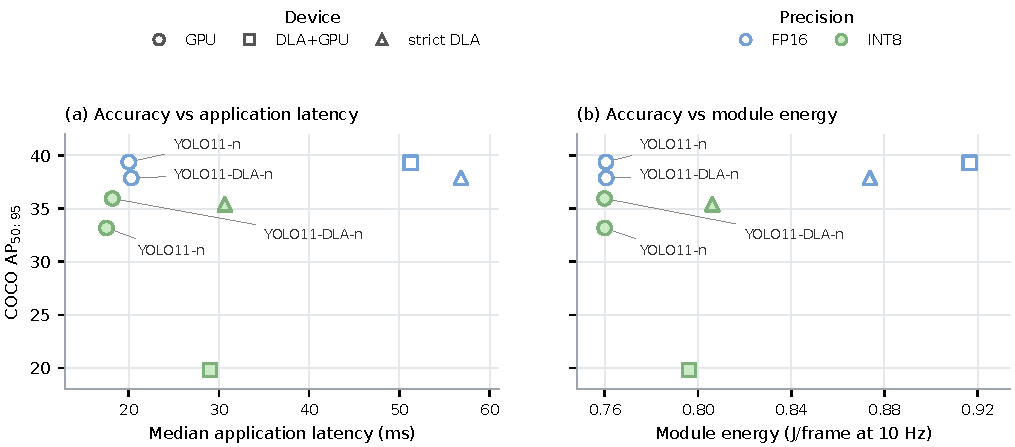
\includegraphics[width=\textwidth]{figures/deployment_tradeoffs.pdf}
\caption{Deployment trade-offs for all eight configurations: held-out COCO AP
versus application latency and module energy at 10\,Hz. Marker shapes identify
GPU, DLA+GPU, and strict DLA deployment; open and filled markers denote FP16
and INT8, respectively. Strict DLA provides verified learned-graph placement
without GPU-assigned learned layers, a property not represented by either
quantitative axis.}
\label{fig:tradeoffs}
\end{figure*}

Module power sums the non-overlapping \texttt{VDD\_GPU\_SOC},
\texttt{VDD\_CPU\_CV}, and \texttt{VIN\_SYS\_5V0} rails, excluding wall-plug
and whole-carrier consumption. Module energy per frame is
\begin{equation}
 E_{\mathrm{frame}}=\frac{\int_{t_0}^{t_1}P_{\mathrm{module}}(t)\,dt}
 {N_{\mathrm{completed}}}.
 \label{eq:energy}
\end{equation}
Separate idle measurements for each precision are subtracted over each active
interval to obtain incremental energy.
The measurement covers the whole module, including the CPU stages around the
accelerator, and is not a measurement of DLA core efficiency.

\begin{table}[t]
\caption{Module energy at 10\,Hz, 600 frames per test. Total and idle-subtracted energy: J/frame.}
\label{tab:energy}\centering\footnotesize
\setlength{\tabcolsep}{3pt}
\begin{tabular*}{\columnwidth}{@{\extracolsep{\fill}}lllrr@{}}
\toprule
Model & Device & Mode & \shortstack{Total\\J/frame} & \shortstack{Idle-subtracted\\J/frame} \\
\midrule
YOLO11-n & GPU & FP16 & 0.761 & 0.060 \\
YOLO11-n & DLA+GPU & FP16 & 0.917 & 0.216 \\
YOLO11-DLA-n & GPU & FP16 & 0.761 & 0.060 \\
YOLO11-DLA-n & DLA & FP16 & 0.874 & 0.174 \\
\midrule
YOLO11-n & GPU & INT8 & 0.760 & 0.060 \\
YOLO11-n & DLA+GPU & INT8 & 0.796 & 0.096 \\
YOLO11-DLA-n & GPU & INT8 & 0.760 & 0.060 \\
YOLO11-DLA-n & DLA & INT8 & 0.806 & 0.106 \\
\bottomrule
\end{tabular*}
\end{table}
Strict INT8 uses 0.806\,J/frame, 7.7\% below strict FP16, but 6.1\% above
adapted INT8 GPU (Table~\ref{tab:energy}). Whereas strict FP16 uses 4.7\% less
energy than stock FP16 fallback, strict INT8 is slightly higher than its
fallback counterpart (0.796\,J/frame), whose accuracy is much lower.
GPU module energy remains approximately 0.760--0.761\,J/frame in both modes.
These results apply to the measured 10\,Hz operating point. Small differences
and idle-subtracted values remain sensitive to baseline stability.

Figure~\ref{fig:tradeoffs} summarizes the deployment trade-offs. For each DLA
configuration, a GPU configuration offers higher AP with lower application
latency and lower module energy. Strict DLA instead provides verified placement
without GPU-assigned learned layers, a property outside these quantitative axes.


\section{Discussion}
\label{sec:discussion}
\subsection{Where the Cost Falls}
Engine gains can shrink or reverse at the application boundary. Strict INT8
is $6.60\times$ faster than strict FP16 at the engine boundary, but only
$1.85\times$ faster in the application pipeline. Its module energy is 7.7\%
lower, and its AP is lower too. Native I/O conversion and host processing limit the application gain.
Adapted INT8 GPU remains faster and lower-energy.

The reversal is a consequence of accelerator speed rather than of its slowness.
At FP16 the strict DLA inference stage dominated its boundaries; at INT8 a
4.522\,ms inference stage does not. Boundary cost becomes the binding constraint
precisely when the accelerator succeeds.

Quantization changes accuracy and runtime behavior. The additional
GPU-to-DLA AP difference grows from 0.003 points in FP16 to 0.543 in INT8.
Stock INT8 fallback has much lower accuracy, with no isolated cause.

\subsection{Scope and Transfer to Other Deployments}
The evidence covers one Jetson/TensorRT configuration and one YOLO11-n case
study. Stock and adapted training budgets differ.
Transfer to other models and DLA configurations is untested.

\section{Conclusion}
Verified fallback-free placement of a modern detector on DLA is achievable, and
at the measured operating point it costs more in the application pipeline than
the same network on GPU, with the boundary rather than the accelerator
accounting for the difference.
For YOLO11, the resulting adaptation combines C2DLA with a static raw prediction boundary;
fallback-disabled compilation and engine inspection verify one DLA loadable
in FP16 and INT8 on the tested Orin/TensorRT stack. FP16 nearly preserves
adapted GPU aggregate AP. Relative to FP16, INT8 reduces strict DLA engine-plus-transfer latency,
application-pipeline latency, and module energy at 10\,Hz, with an accuracy cost.
Adapted GPU remains faster and lower-energy at this operating point.

The case study shows that DLA adaptation is not only an operator-replacement
problem. The prediction boundary, tensor layouts, host processing, and placement
checks also matter. Concurrent robotic workloads remain outside this evaluation. Whether removing
the learned detector from GPU compute benefits them is the open question this
case study raises but does not answer: the measured 7--10\% GR3D utilization
shows the GPU is not idle during strict execution, and the strict configuration
occupies the platform for longer per frame, so a system-level test with a
competing workload is required before any such benefit can be claimed.
Other models and DLA configurations require their own validation.


\bibliographystyle{IEEEtran}
\bibliography{references}

\end{document}
